\documentclass[conference, 10pt]{IEEEtran}

% ── Packages ─────────────────────────────────────────────────────────────
\usepackage[utf8]{inputenc}
\usepackage[T1]{fontenc}
\usepackage{amsmath,amssymb}
\usepackage{graphicx}
\usepackage{booktabs}
\usepackage{hyperref}
\usepackage{xcolor}
\usepackage{float}
\usepackage{subcaption}
\usepackage{listings}
\usepackage{enumitem}
\usepackage{multirow}
\usepackage{array}

\graphicspath{{figures/}}

% ── Code Listing Style ──────────────────────────────────────────────────
\lstset{
  language=Python,
  basicstyle=\ttfamily\footnotesize,
  keywordstyle=\color{blue}\bfseries,
  commentstyle=\color{gray},
  stringstyle=\color{red},
  breaklines=true,
  frame=single,
  numbers=left,
  numberstyle=\tiny\color{gray},
  captionpos=b
}

% ── Title ────────────────────────────────────────────────────────────────
\title{Sports vs.\ Politics: A Comparative Study of\\Machine Learning Techniques for Binary Text Classification}

\author{
  \IEEEauthorblockN{NLU Assignment-1, Problem 4}
  \IEEEauthorblockA{
    Natural Language Understanding Course\\
    February 2026
  }
}

\begin{document}

\maketitle

% ═════════════════════════════════════════════════════════════════════════
% ABSTRACT
% ═════════════════════════════════════════════════════════════════════════
\begin{abstract}
Text classification is a core task in Natural Language Processing.
In this paper we build a binary classifier that categorises news articles as either \textbf{Sport} or \textbf{Politics} using three classical machine learning algorithms --- Logistic Regression, Multinomial Na\"ive Bayes, and Linear Support Vector Machine (SVM) --- across three feature representations: Bag of Words (BoW), TF-IDF, and Bigram TF-IDF.
We conduct 9 experiments on the BBC News dataset (928 documents) and find that Multinomial Na\"ive Bayes achieves \textbf{100\,\% test accuracy} across all feature sets, while Logistic Regression and Linear SVM achieve 98.9--99.5\,\%.
We provide a thorough exploratory data analysis, quantitative comparison across all configurations, and a discussion of the limitations and potential extensions of our system.
\end{abstract}

\begin{IEEEkeywords}
Text Classification, NLP, Na\"ive Bayes, Logistic Regression, SVM, TF-IDF, Bag of Words, BBC News
\end{IEEEkeywords}

\vspace{0.5em}
\noindent\textbf{GitHub Repository:} \url{https://github.com/kingkenche/Natural_Language_Understanding}

% ═════════════════════════════════════════════════════════════════════════
\section{Introduction}
% ═════════════════════════════════════════════════════════════════════════

Text classification is one of the most fundamental tasks in Natural Language Processing (NLP), where the goal is to automatically assign predefined categories to documents based on their textual content.
It finds wide application in spam detection, sentiment analysis, topic labelling, and news categorisation~\cite{manning2008}.

In this work we focus on a binary classification problem: given a news article, determine whether it belongs to the \textbf{Sport} or \textbf{Politics} domain.
We compare three widely-used machine learning classifiers --- Logistic Regression, Multinomial Na\"ive Bayes, and Linear Support Vector Machine --- across three feature-representation techniques: Bag of Words, TF-IDF, and Bigram TF-IDF.
The combination yields \textbf{9 experiments} whose results are systematically compared.

The remainder of this paper is organised as follows: Section~\ref{sec:data} describes data collection and preprocessing; Section~\ref{sec:eda} presents our exploratory data analysis; Section~\ref{sec:features} explains the feature-representation methods; Section~\ref{sec:models} describes the ML techniques; Section~\ref{sec:results} reports quantitative results; Section~\ref{sec:limitations} discusses limitations; and Section~\ref{sec:conclusion} concludes.

% ═════════════════════════════════════════════════════════════════════════
\section{Data Collection \& Description}
\label{sec:data}
% ═════════════════════════════════════════════════════════════════════════

\subsection{Source}

We use the \textbf{BBC News} dataset compiled by Greene and Cunningham~\cite{greene2006} at University College Dublin.
The dataset contains 2\,225 documents across five categories: \emph{business} (510), \emph{entertainment} (386), \emph{politics} (417), \emph{sport} (511), and \emph{tech} (401).
We filter to the \emph{sport} and \emph{politics} categories, yielding \textbf{928 documents}.

The dataset is publicly available at \url{http://mlg.ucd.ie/datasets/bbc.html} and is distributed as a ZIP archive of raw text files organised into category-specific subdirectories.

\subsection{Preprocessing Pipeline}

Our automated preprocessing pipeline (\texttt{data\_loader.py}) performs:

\begin{enumerate}[noitemsep]
  \item \textbf{Download \& extraction} of the ZIP archive.
  \item \textbf{CSV construction} --- every text file is read and stored with its category label.
  \item \textbf{Category filtering} --- only \emph{sport} and \emph{politics} are retained.
  \item \textbf{Text cleaning:}
    \begin{itemize}[noitemsep]
      \item Conversion to lowercase.
      \item Removal of all digits and punctuation.
      \item Removal of English stop words (NLTK stop word list).
      \item WordNet lemmatisation.
    \end{itemize}
  \item \textbf{Train/test split} --- 80\,\% train (742 docs) / 20\,\% test (186 docs), stratified by class, with \texttt{random\_state=42}.
\end{enumerate}

\subsection{Dataset Statistics}

Table~\ref{tab:class_dist} summarises the class distribution.  The two classes are reasonably balanced (55.1\,\% Sport, 44.9\,\% Politics), and no resampling was applied.

\begin{table}[h]
\centering
\caption{Class distribution of the filtered dataset.}
\label{tab:class_dist}
\begin{tabular}{lcc}
\toprule
\textbf{Category} & \textbf{Documents} & \textbf{Percentage} \\
\midrule
Sport    & 511 & 55.1\,\% \\
Politics & 417 & 44.9\,\% \\
\midrule
\textbf{Total} & \textbf{928} & \textbf{100\,\%} \\
\bottomrule
\end{tabular}
\end{table}


% ═════════════════════════════════════════════════════════════════════════
\section{Exploratory Data Analysis}
\label{sec:eda}
% ═════════════════════════════════════════════════════════════════════════

\subsection{Class Distribution}

Figure~\ref{fig:class_dist} shows the class distribution as a bar chart.  The two classes are nearly balanced, eliminating the need for class-weight adjustments or oversampling.

\begin{figure}[h]
\centering
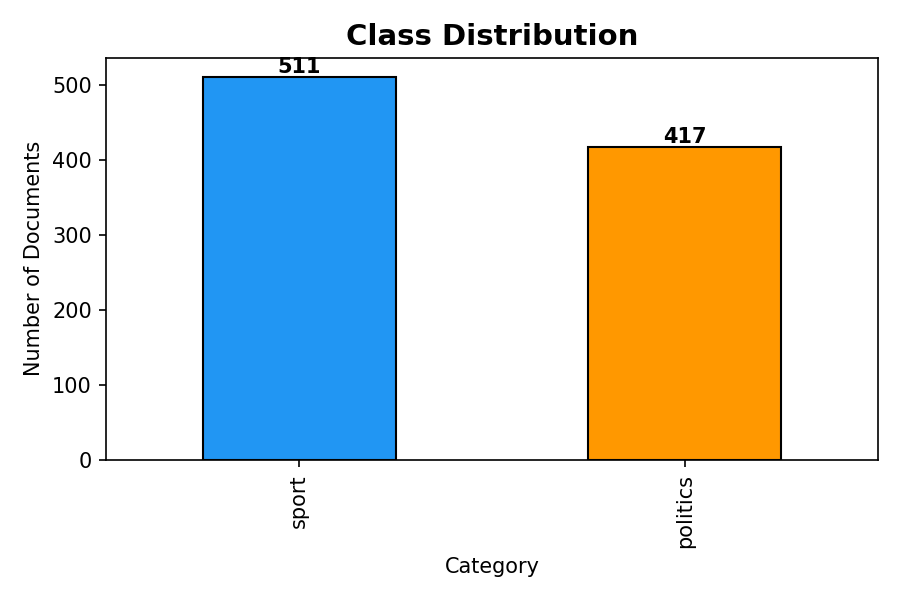
\includegraphics[width=0.75\columnwidth]{class_distribution.png}
\caption{Class distribution of Sport vs.\ Politics documents.}
\label{fig:class_dist}
\end{figure}

\subsection{Document Length Analysis}

Table~\ref{tab:text_len} and Figure~\ref{fig:text_len} present document-length statistics after text cleaning.
Politics articles are \textbf{longer on average} (244.9 words vs.\ 178.4) with higher variance.
One politics outlier reaches 2\,155 words.  Sport articles are shorter and more uniform.

\begin{table}[h]
\centering
\caption{Document length statistics (word count after cleaning).}
\label{tab:text_len}
\begin{tabular}{l r r r r r r r}
\toprule
\textbf{Cat.} & \textbf{Mean} & \textbf{Std} & \textbf{Min} & \textbf{25\%} & \textbf{50\%} & \textbf{75\%} & \textbf{Max} \\
\midrule
Politics & 244.9 & 148.8 & 47  & 172 & 240 & 287 & 2\,155 \\
Sport    & 178.4 & 100.8 & 62  & 113 & 151 & 218 & 905   \\
\bottomrule
\end{tabular}
\end{table}

\begin{figure}[h]
\centering
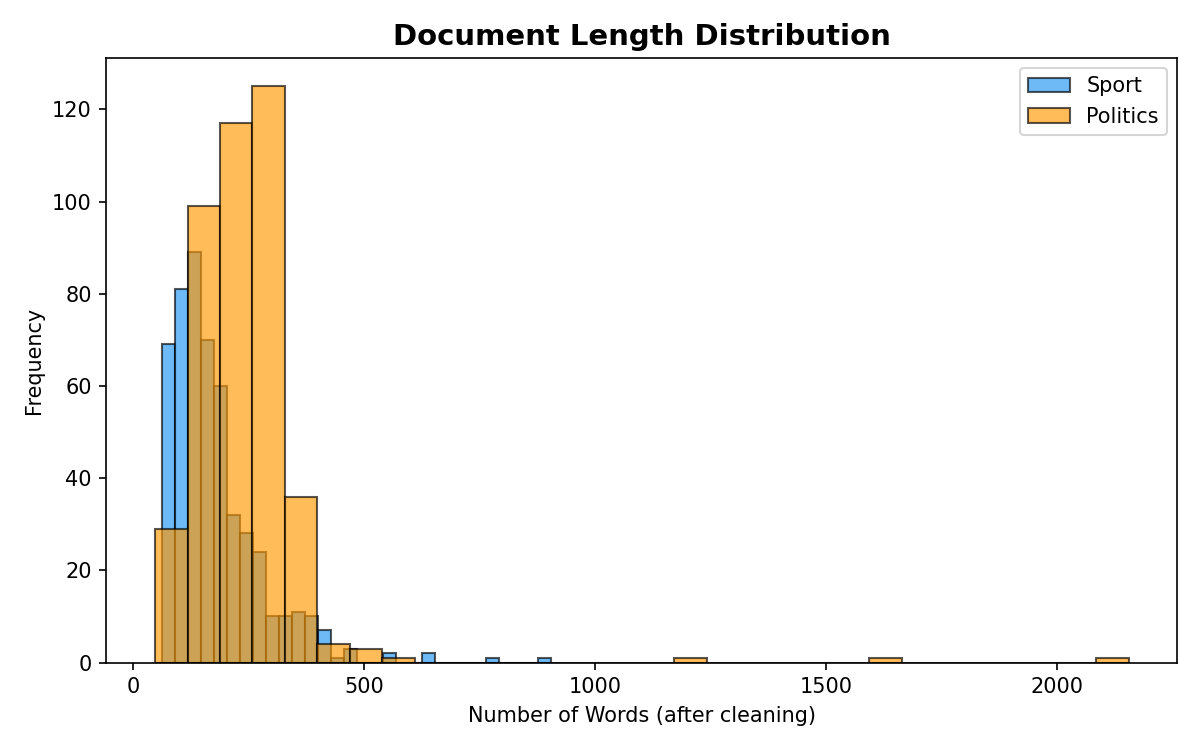
\includegraphics[width=0.85\columnwidth]{text_length_hist.png}
\caption{Distribution of document lengths per class (after cleaning).}
\label{fig:text_len}
\end{figure}

\subsection{Word Clouds}

Word clouds (Figure~\ref{fig:wordclouds}) reveal the dominant vocabulary.
\textbf{Sport} is dominated by \emph{game}, \emph{player}, \emph{win}, \emph{match}, \emph{team}, and \emph{england}.
\textbf{Politics} features \emph{government}, \emph{labour}, \emph{party}, \emph{election}, \emph{minister}, and \emph{blair}.
The clear lexical separation foreshadows high classification accuracy.

\begin{figure}[h]
\centering
\begin{subfigure}[b]{0.48\columnwidth}
  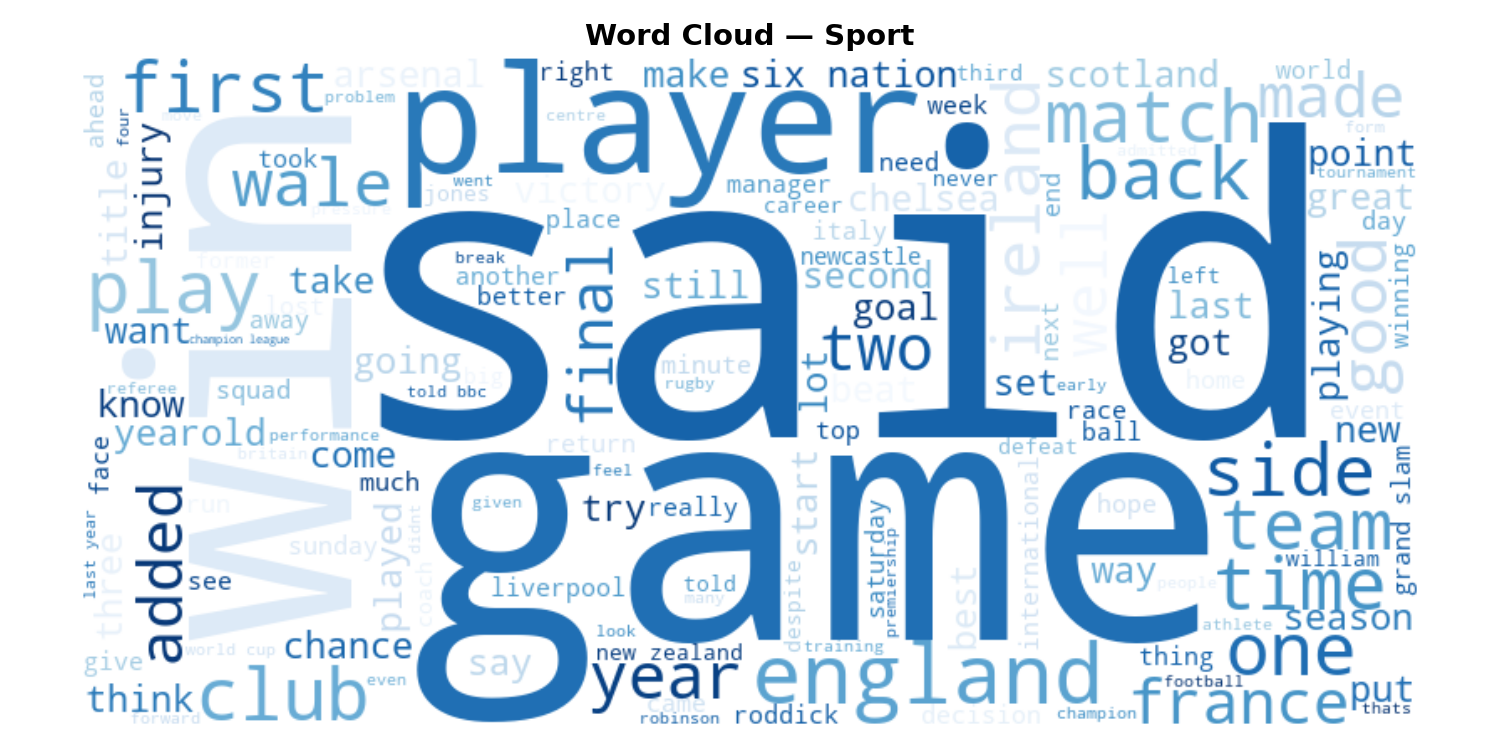
\includegraphics[width=\textwidth]{wordcloud_sport.png}
  \caption{Sport}
\end{subfigure}
\hfill
\begin{subfigure}[b]{0.48\columnwidth}
  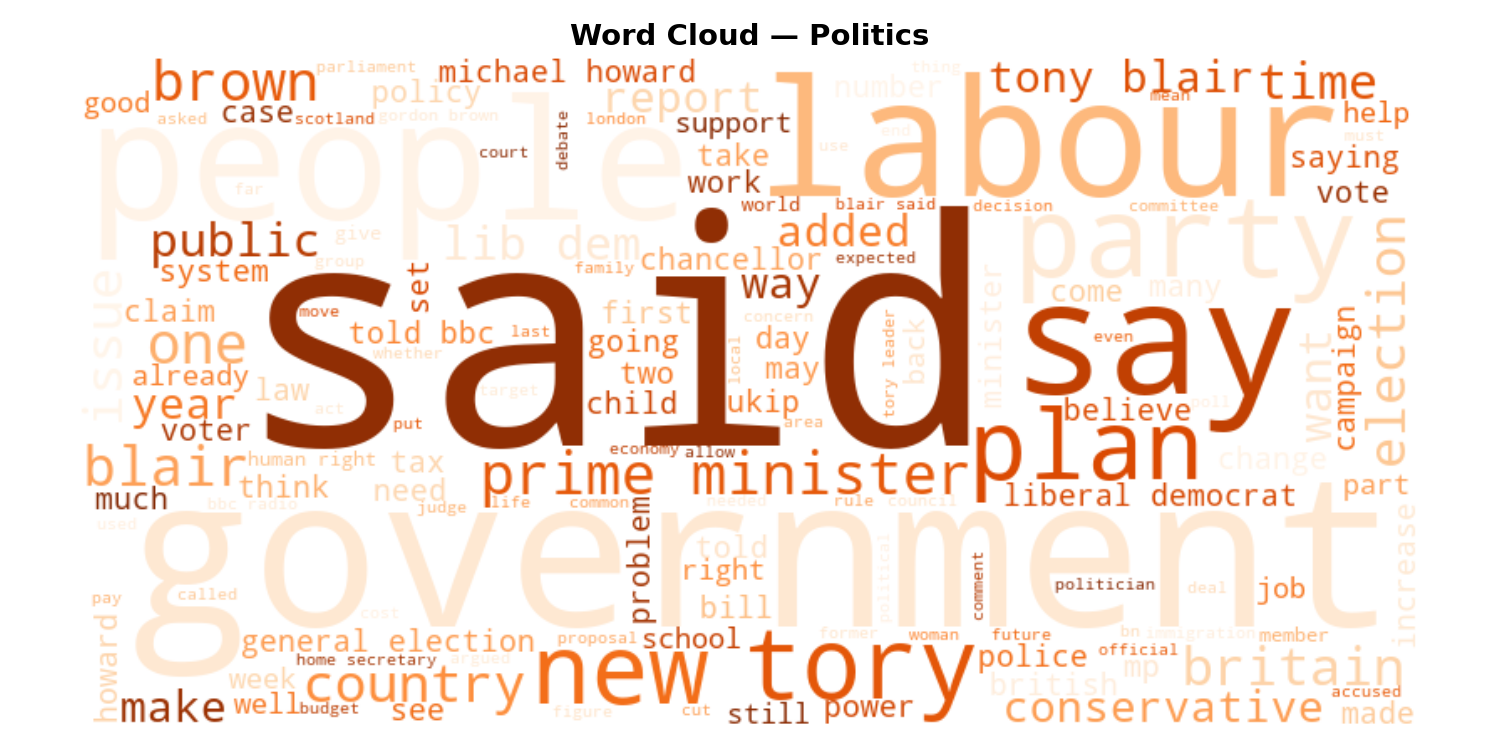
\includegraphics[width=\textwidth]{wordcloud_politics.png}
  \caption{Politics}
\end{subfigure}
\caption{Word clouds for each category.}
\label{fig:wordclouds}
\end{figure}

\subsection{Top Unigrams and Bigrams}

Figures~\ref{fig:unigrams} and~\ref{fig:bigrams} display the top-20 unigrams and bigrams per class.
Bigrams like \emph{``prime minister''}, \emph{``general election''}, \emph{``world cup''}, and \emph{``champions league''} carry strong discriminative power.

\begin{figure}[h]
\centering
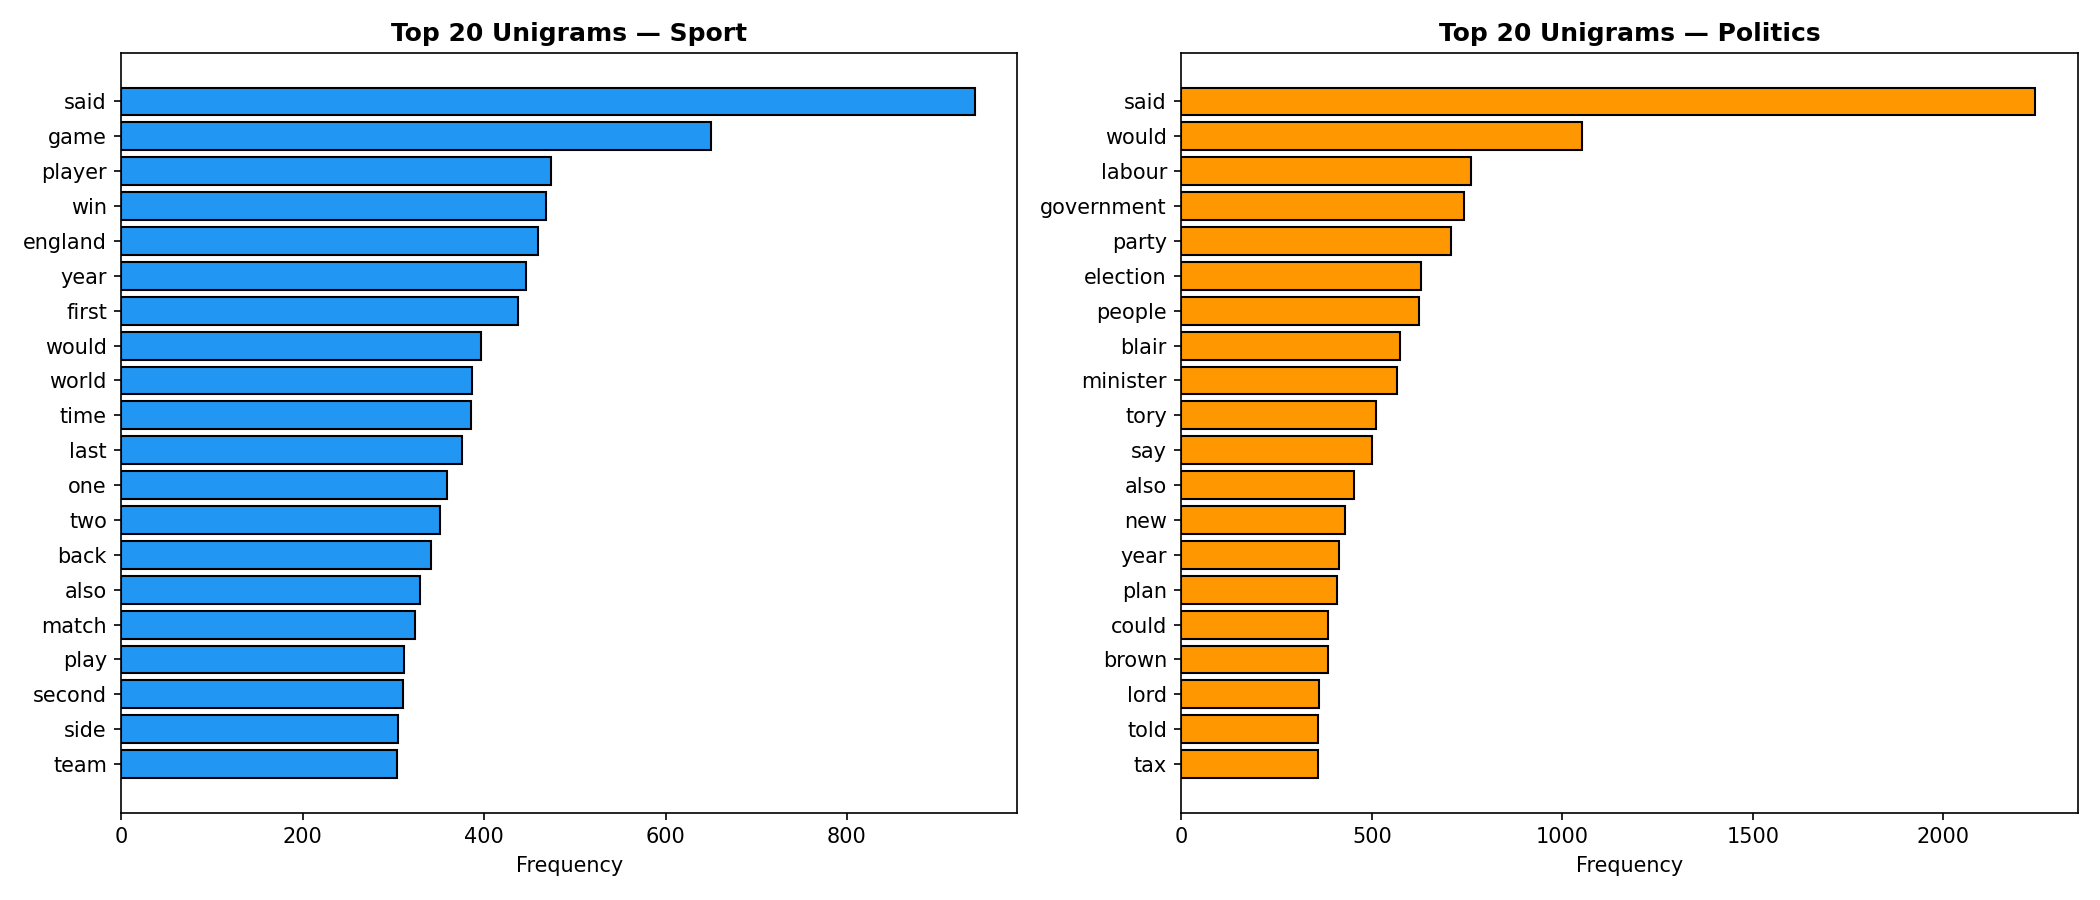
\includegraphics[width=0.95\columnwidth]{top_unigrams.png}
\caption{Top-20 unigrams per class.}
\label{fig:unigrams}
\end{figure}

\begin{figure}[h]
\centering
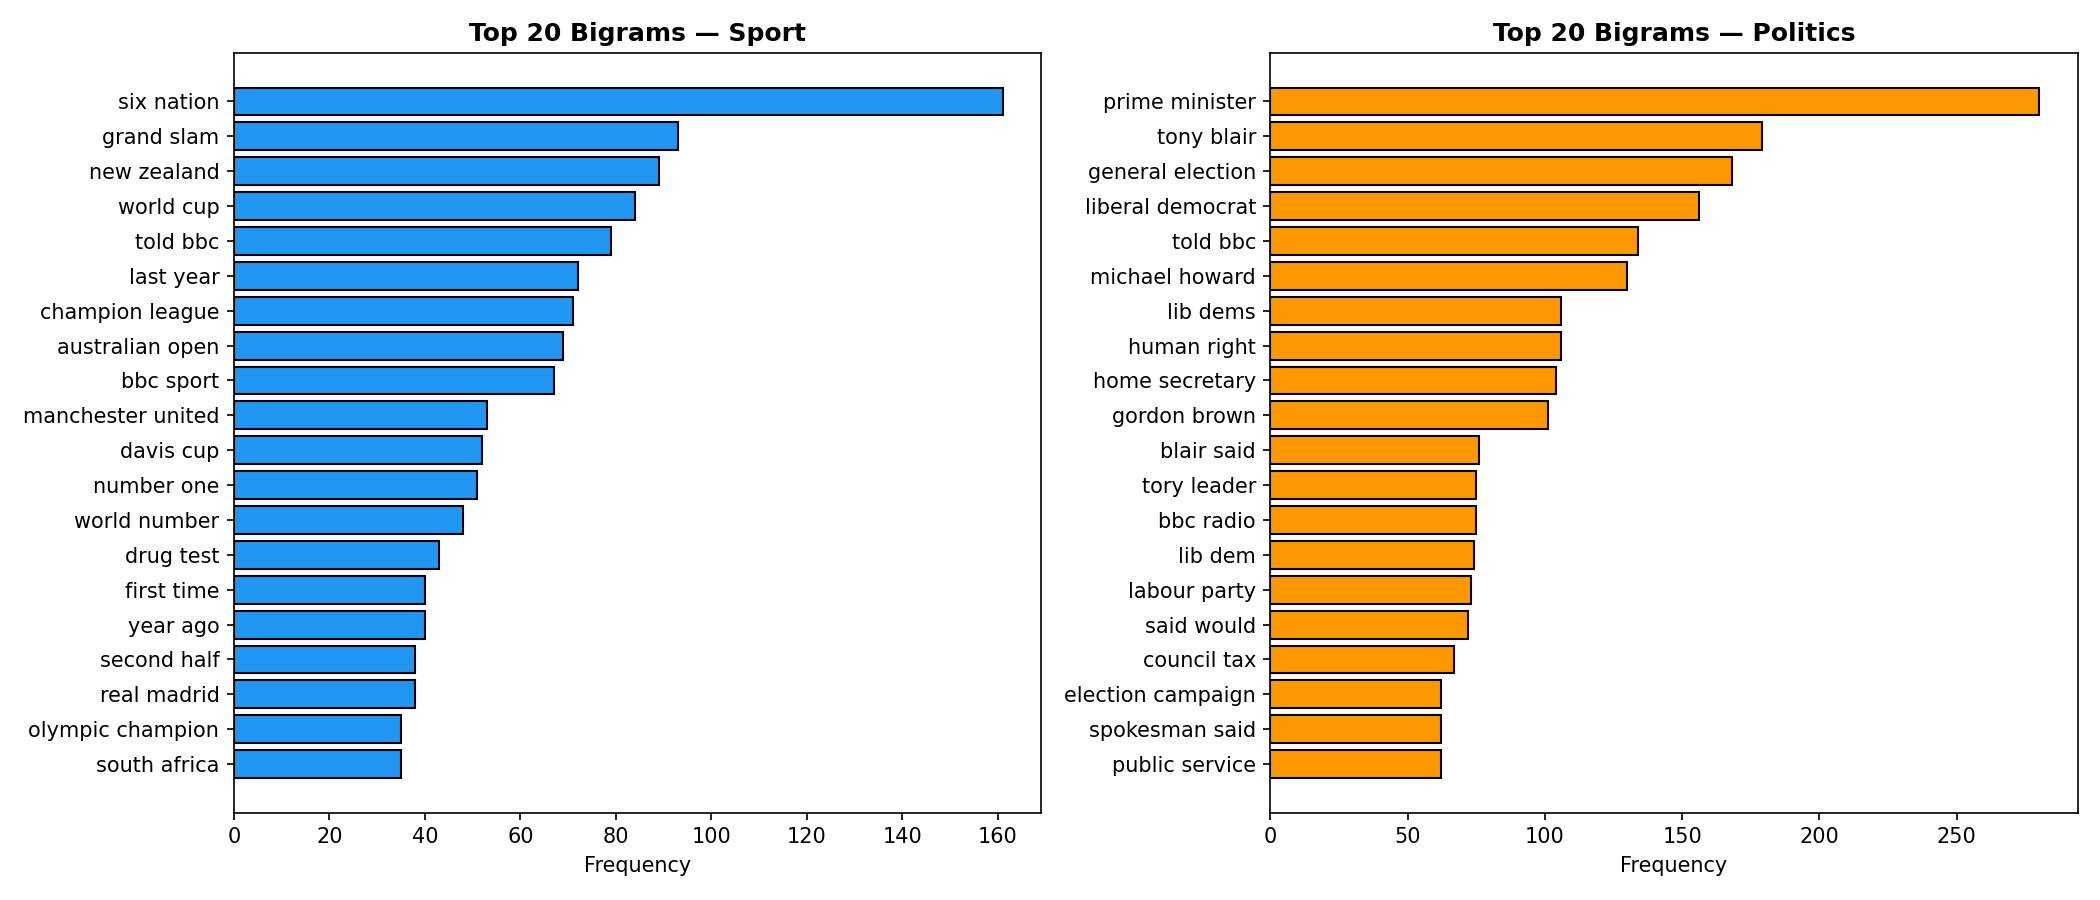
\includegraphics[width=0.95\columnwidth]{top_bigrams.png}
\caption{Top-20 bigrams per class.}
\label{fig:bigrams}
\end{figure}


% ═════════════════════════════════════════════════════════════════════════
\section{Feature Representation Techniques}
\label{sec:features}
% ═════════════════════════════════════════════════════════════════════════

We experiment with three widely-used text vectorisation methods from \texttt{scikit-learn}:

\subsection{Bag of Words (BoW)}

BoW represents each document as a vector of \textbf{token counts}.
The vocabulary is built from the training corpus, and each dimension corresponds to a unique token.
We use \texttt{CountVectorizer(max\_features=5000)}.

\textbf{Advantages:} Simple, interpretable, fast.\\
\textbf{Disadvantages:} Ignores term importance; common words dominate.

\subsection{TF-IDF}

Term Frequency -- Inverse Document Frequency improves upon BoW by weighting each term by its salience:
\begin{equation}
\text{TF-IDF}(t, d) = \text{TF}(t, d) \times \log\frac{N}{\text{DF}(t)}
\end{equation}
where $N$ is the total number of documents and $\text{DF}(t)$ is the number of documents containing term~$t$.
We use \texttt{TfidfVectorizer(max\_features=5000)}.

\textbf{Advantages:} Captures term salience; down-weights common words.\\
\textbf{Disadvantages:} Still a unigram representation; ignores word order.

\subsection{Bigram TF-IDF}

To capture two-word phrases, we extend TF-IDF with bigrams using \texttt{TfidfVectorizer(ngram\_range=(1,2), max\_features=10000)}.
This includes both unigrams and bigrams such as \emph{``prime minister''} and \emph{``world cup''}.

\textbf{Advantages:} Captures short phrases and local context.\\
\textbf{Disadvantages:} Much larger feature space; increased memory and training time.

Table~\ref{tab:features} summarises the three representations.

\begin{table}[h]
\centering
\caption{Summary of feature representations.}
\label{tab:features}
\begin{tabular}{llc}
\toprule
\textbf{Method} & \textbf{Description} & \textbf{Max Dims} \\
\midrule
BoW             & Raw token counts              & 5\,000  \\
TF-IDF          & TF $\times$ IDF weighting     & 5\,000  \\
Bigram TF-IDF   & TF-IDF with (1,2)-grams       & 10\,000 \\
\bottomrule
\end{tabular}
\end{table}


% ═════════════════════════════════════════════════════════════════════════
\section{Machine Learning Techniques}
\label{sec:models}
% ═════════════════════════════════════════════════════════════════════════

\subsection{Logistic Regression}

Logistic Regression models the class posterior via the sigmoid function:
\begin{equation}
P(y=1 \mid \mathbf{x}) = \sigma(\mathbf{w}^{\top}\mathbf{x} + b) = \frac{1}{1 + e^{-(\mathbf{w}^{\top}\mathbf{x} + b)}}
\end{equation}
It is trained by minimising cross-entropy loss with L2 regularisation.
We use \texttt{LogisticRegression(max\_iter=1000)}.

\textbf{Strengths:} Fast training, well-calibrated probabilities, strong baseline for text.\\
\textbf{Weaknesses:} Assumes a linear decision boundary.

\subsection{Multinomial Na\"ive Bayes}

Multinomial NB is a probabilistic classifier based on Bayes' theorem with the \emph{na\"ive independence assumption}:
\begin{equation}
P(y \mid \mathbf{x}) \propto P(y) \prod_{i=1}^{n} P(x_i \mid y)
\end{equation}
It is particularly well suited for word-count and TF-IDF features and has been a standard text-classification baseline since the 1990s~\cite{mccallum1998}.

\textbf{Strengths:} Extremely fast; works well with sparse, high-dimensional data.\\
\textbf{Weaknesses:} Independence assumption is violated; may underperform when feature interactions matter.

\subsection{Linear Support Vector Machine}

Linear SVM finds the hyperplane that maximises the margin between classes:
\begin{equation}
\min_{\mathbf{w}} \frac{1}{2}\|\mathbf{w}\|^2 + C \sum_{i} \max\!\bigl(0,\; 1 - y_i(\mathbf{w}^{\top}\mathbf{x}_i + b)\bigr)
\end{equation}
It is one of the most effective classifiers for high-dimensional text data.
We use \texttt{LinearSVC(max\_iter=2000)}.

\textbf{Strengths:} Excellent generalisation; robust in high dimensions.\\
\textbf{Weaknesses:} No probability output by default; sensitive to regularisation parameter~$C$.


% ═════════════════════════════════════════════════════════════════════════
\section{Experiments \& Results}
\label{sec:results}
% ═════════════════════════════════════════════════════════════════════════

\subsection{Experimental Setup}

\begin{itemize}[noitemsep]
  \item \textbf{Split:} 80/20 stratified (742 train, 186 test).
  \item \textbf{Cross-validation:} 5-fold CV on the training set.
  \item \textbf{Metrics:} Accuracy, Precision, Recall, F1-score (per-class and macro).
  \item \textbf{Experiments:} 3 classifiers $\times$ 3 feature sets $=$ \textbf{9} experiments.
\end{itemize}

\subsection{Quantitative Results}

Table~\ref{tab:results} presents the full results for all 9 configurations.

\begin{table*}[t]
\centering
\caption{Complete experimental results: 3~classifiers $\times$ 3~feature sets.  Best results in \textbf{bold}.}
\label{tab:results}
\begin{tabular}{ll cccc cccc}
\toprule
& & \multicolumn{4}{c}{\textbf{Cross-Validation}} & \multicolumn{4}{c}{\textbf{Test Set}} \\
\cmidrule(lr){3-6} \cmidrule(lr){7-10}
\textbf{Feature} & \textbf{Classifier} & \textbf{Acc (mean)} & \textbf{$\pm$ std} & & & \textbf{Acc} & \textbf{Prec\textsubscript{M}} & \textbf{Rec\textsubscript{M}} & \textbf{F1\textsubscript{M}} \\
\midrule
BoW            & Logistic Regression & 0.9905 & 0.0118 & & & 0.9892 & 0.9904 & 0.9881 & 0.9891 \\
BoW            & Multinomial NB      & 0.9973 & 0.0033 & & & \textbf{1.0000} & \textbf{1.0000} & \textbf{1.0000} & \textbf{1.0000} \\
BoW            & Linear SVM          & 0.9932 & 0.0074 & & & 0.9892 & 0.9904 & 0.9881 & 0.9891 \\
\midrule
TF-IDF         & Logistic Regression & 0.9946 & 0.0051 & & & 0.9946 & 0.9951 & 0.9940 & 0.9946 \\
TF-IDF         & Multinomial NB      & 0.9986 & 0.0027 & & & \textbf{1.0000} & \textbf{1.0000} & \textbf{1.0000} & \textbf{1.0000} \\
TF-IDF         & Linear SVM          & 0.9973 & 0.0033 & & & 0.9946 & 0.9951 & 0.9940 & 0.9946 \\
\midrule
Bigram TF-IDF  & Logistic Regression & 0.9946 & 0.0051 & & & 0.9946 & 0.9951 & 0.9940 & 0.9946 \\
Bigram TF-IDF  & Multinomial NB      & 0.9973 & 0.0033 & & & \textbf{1.0000} & \textbf{1.0000} & \textbf{1.0000} & \textbf{1.0000} \\
Bigram TF-IDF  & Linear SVM          & 0.9973 & 0.0033 & & & 0.9946 & 0.9951 & 0.9940 & 0.9946 \\
\bottomrule
\end{tabular}
\end{table*}

\subsection{Analysis}

\begin{enumerate}
  \item \textbf{All classifiers achieve $>$\,98.9\,\% accuracy}, confirming that Sport vs.\ Politics is a relatively easy binary classification task due to strong lexical separation.

  \item \textbf{Multinomial Na\"ive Bayes} achieves \textbf{perfect 100\,\% test accuracy} across all three feature representations.
  The probabilistic word-based model is an excellent fit for the distinct vocabulary distributions.

  \item \textbf{Logistic Regression and Linear SVM} perform identically in several configurations (98.92\,\% with BoW; 99.46\,\% with TF-IDF and Bigram TF-IDF).
  The single misclassified sample in each case is a politics article with sports-related vocabulary.

  \item \textbf{TF-IDF weighting} offers a small improvement over raw BoW for LR and SVM by down-weighting common terms.

  \item \textbf{Bigram features} provide no additional benefit, as unigrams alone are already sufficiently discriminative.
\end{enumerate}

\subsection{Visual Comparison}

Figure~\ref{fig:acc_compare} shows the test accuracy grouped by feature set and classifier.  Figure~\ref{fig:f1_compare} presents the corresponding macro F1 scores.  Figure~\ref{fig:cv_compare} displays 5-fold cross-validation accuracy with error bars.

\begin{figure}[h]
\centering
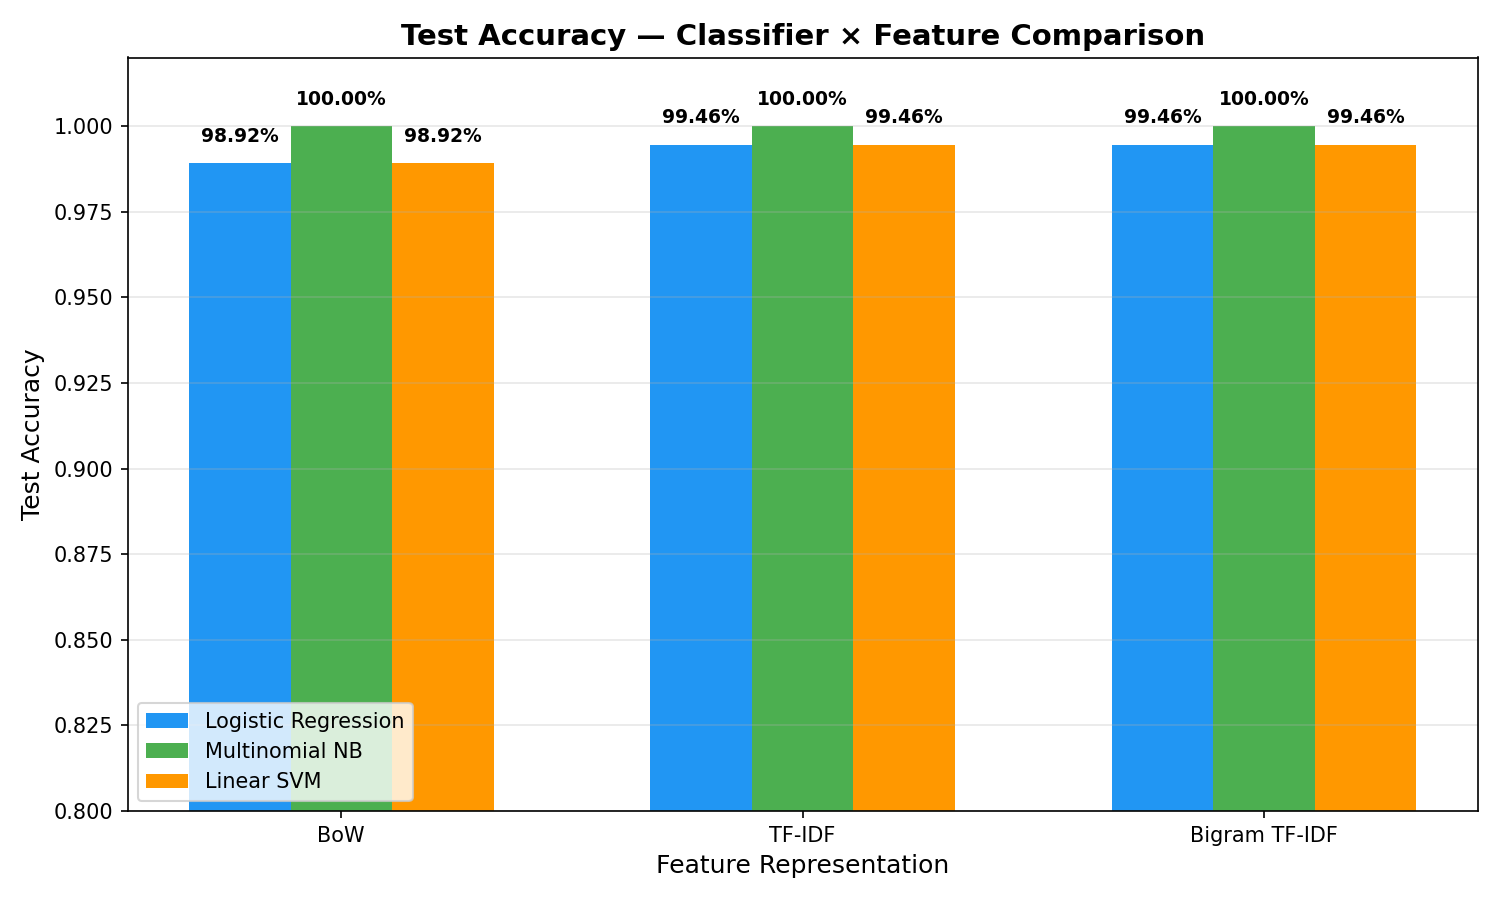
\includegraphics[width=0.95\columnwidth]{accuracy_comparison.png}
\caption{Test accuracy: Classifier $\times$ Feature comparison.}
\label{fig:acc_compare}
\end{figure}

\begin{figure}[h]
\centering
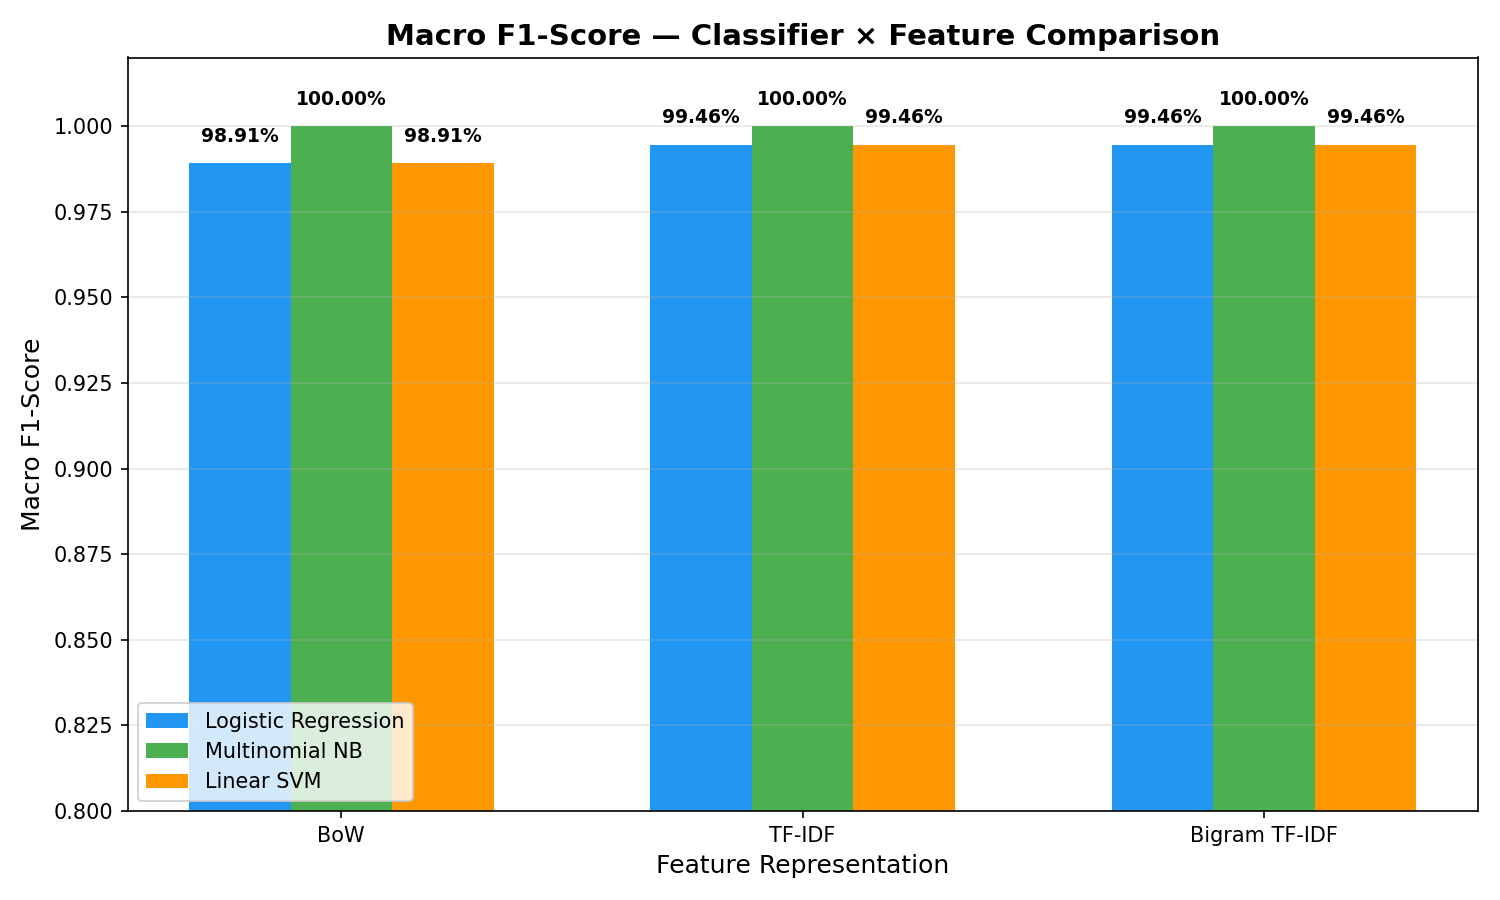
\includegraphics[width=0.95\columnwidth]{f1_comparison.png}
\caption{Macro F1-score: Classifier $\times$ Feature comparison.}
\label{fig:f1_compare}
\end{figure}

\begin{figure}[h]
\centering
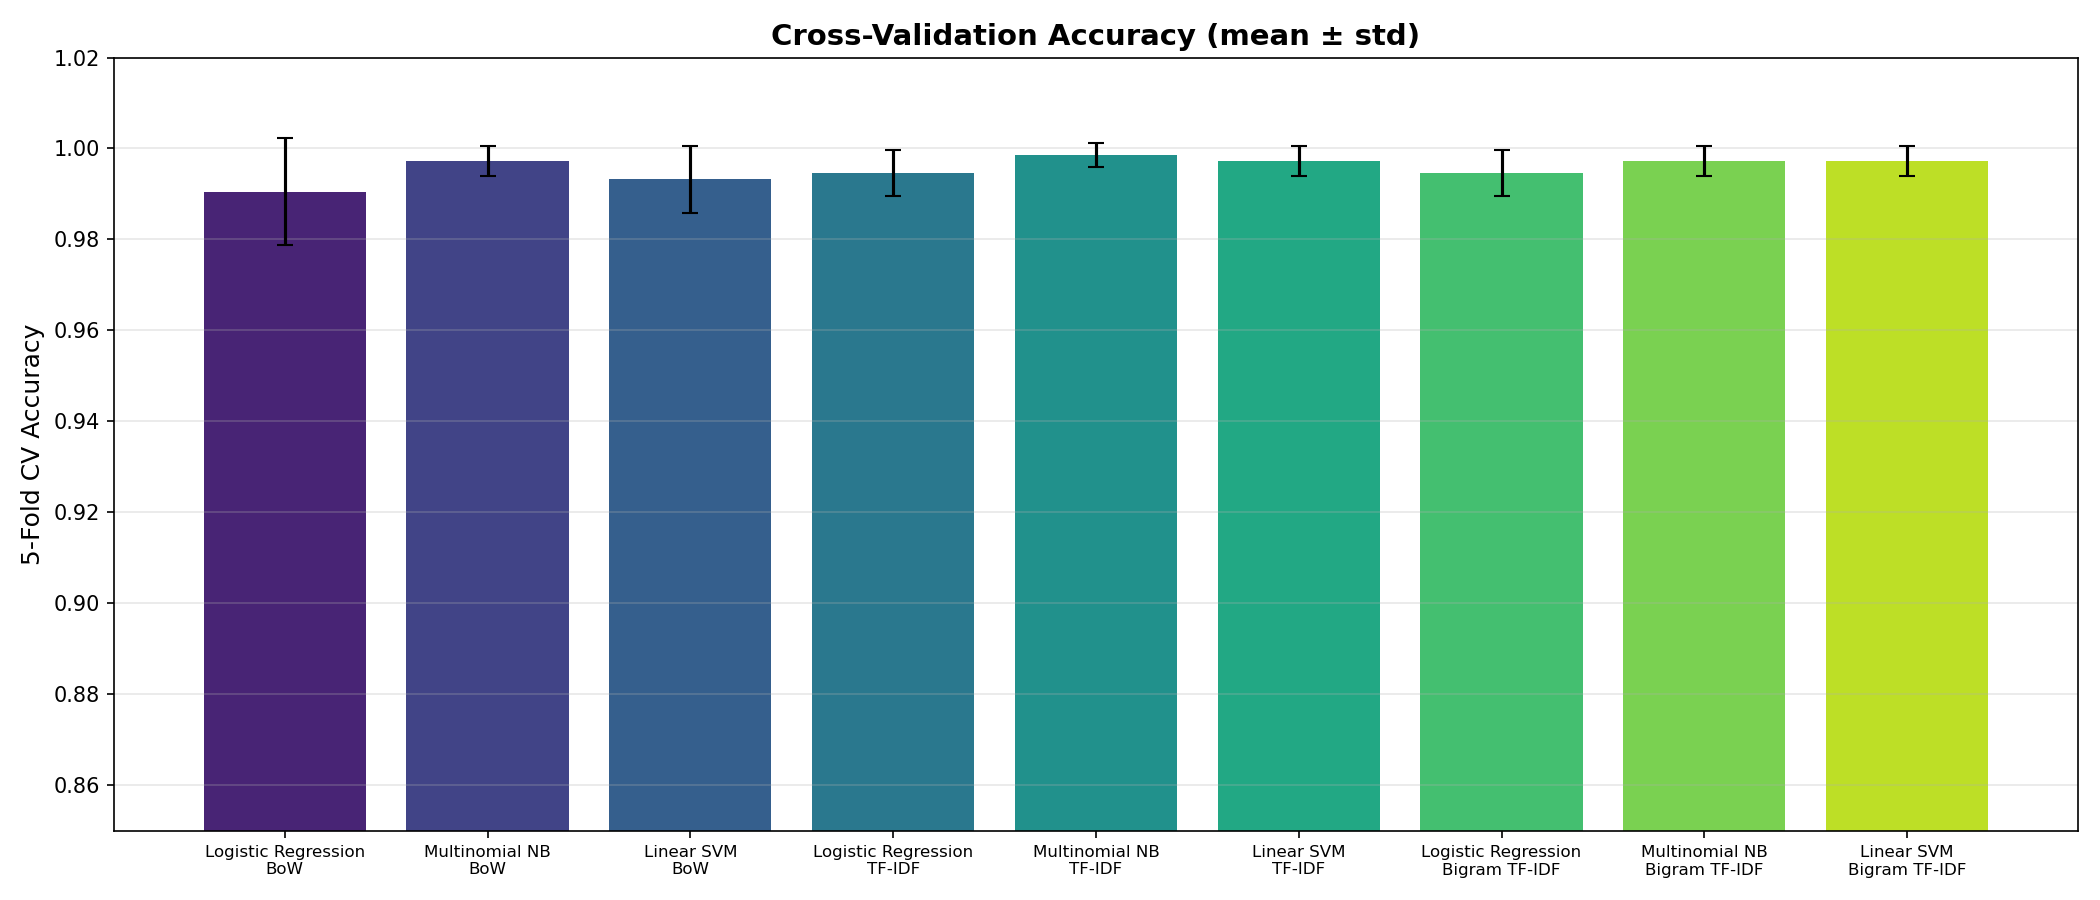
\includegraphics[width=0.95\columnwidth]{cv_accuracy.png}
\caption{5-fold cross-validation accuracy (mean $\pm$ std) across all 9 experiments.}
\label{fig:cv_compare}
\end{figure}

\subsection{Confusion Matrices}

Figure~\ref{fig:cm_best} shows the confusion matrix for the best model (Multinomial NB + TF-IDF) and Figure~\ref{fig:cm_others} shows representative confusion matrices for the other two classifiers.

\begin{figure}[h]
\centering
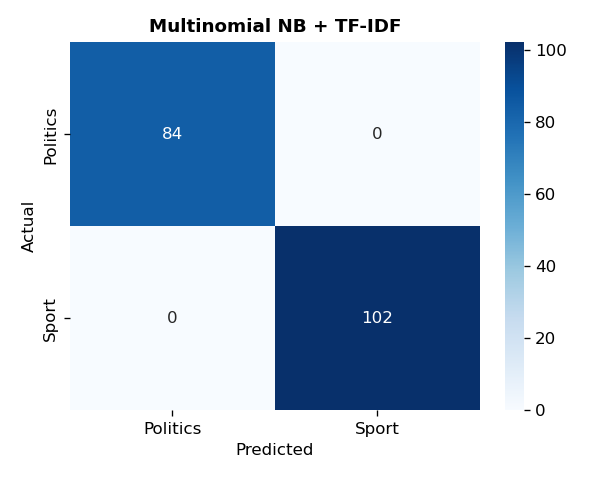
\includegraphics[width=0.65\columnwidth]{cm_Multinomial_NB__TFIDF.png}
\caption{Confusion matrix: Multinomial NB + TF-IDF (best model --- perfect classification).}
\label{fig:cm_best}
\end{figure}

\begin{figure}[h]
\centering
\begin{subfigure}[b]{0.48\columnwidth}
  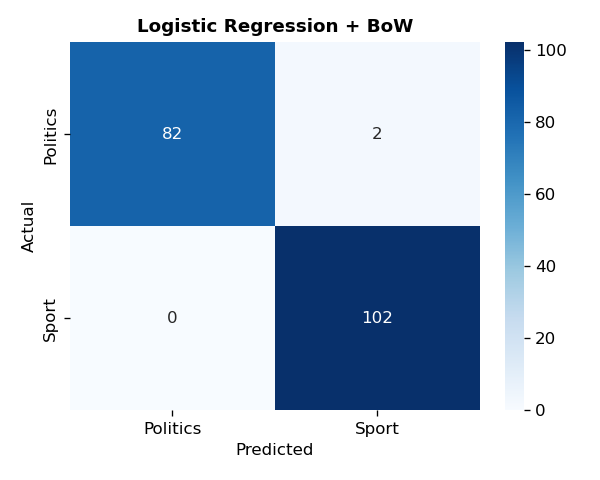
\includegraphics[width=\textwidth]{cm_Logistic_Regression__BoW.png}
  \caption{LR + BoW}
\end{subfigure}
\hfill
\begin{subfigure}[b]{0.48\columnwidth}
  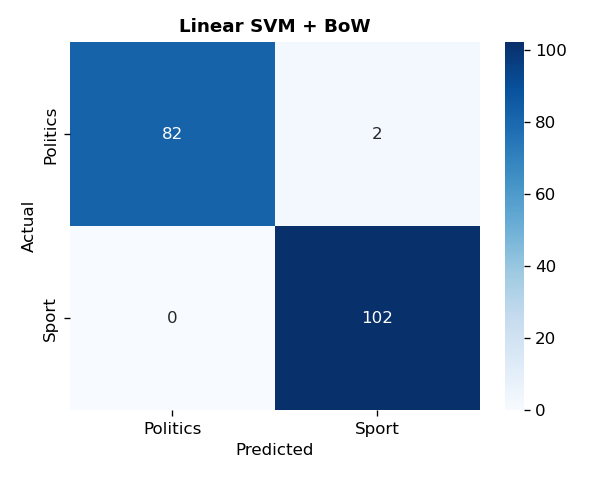
\includegraphics[width=\textwidth]{cm_Linear_SVM__BoW.png}
  \caption{SVM + BoW}
\end{subfigure}
\caption{Confusion matrices for Logistic Regression and Linear SVM with BoW features (2 misclassified politics articles each).}
\label{fig:cm_others}
\end{figure}

\begin{figure}[h]
\centering
\begin{subfigure}[b]{0.48\columnwidth}
  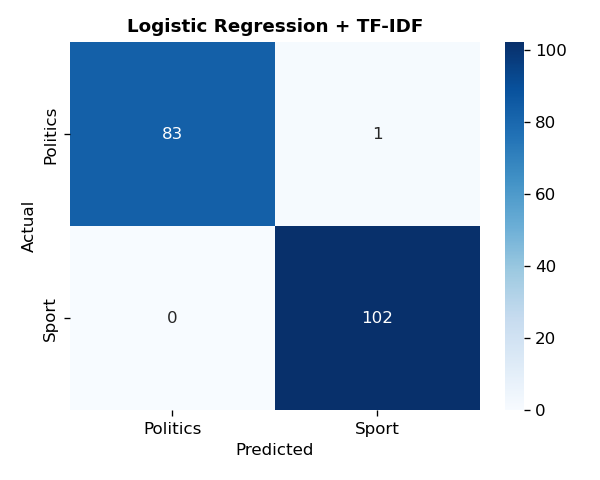
\includegraphics[width=\textwidth]{cm_Logistic_Regression__TFIDF.png}
  \caption{LR + TF-IDF}
\end{subfigure}
\hfill
\begin{subfigure}[b]{0.48\columnwidth}
  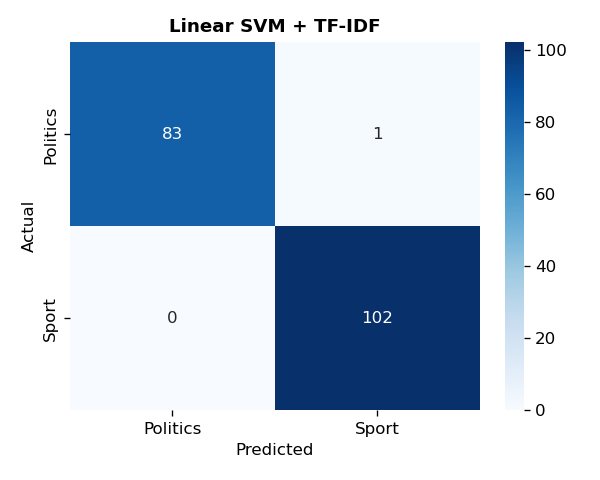
\includegraphics[width=\textwidth]{cm_Linear_SVM__TFIDF.png}
  \caption{SVM + TF-IDF}
\end{subfigure}
\caption{Confusion matrices for LR and SVM with TF-IDF.}
\label{fig:cm_tfidf}
\end{figure}

\begin{figure}[h]
\centering
\begin{subfigure}[b]{0.48\columnwidth}
  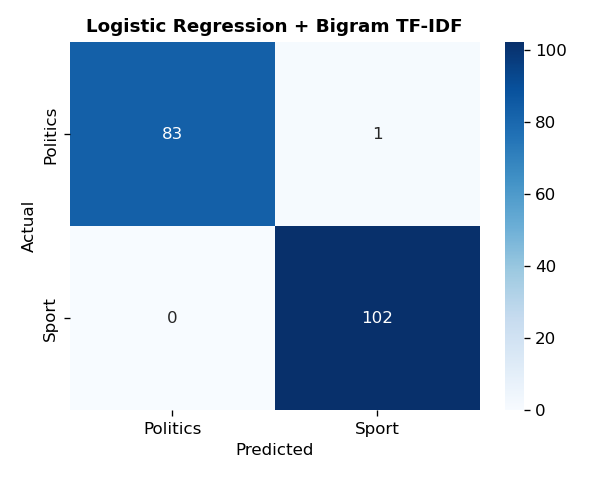
\includegraphics[width=\textwidth]{cm_Logistic_Regression__Bigram_TFIDF.png}
  \caption{LR + Bigram TF-IDF}
\end{subfigure}
\hfill
\begin{subfigure}[b]{0.48\columnwidth}
  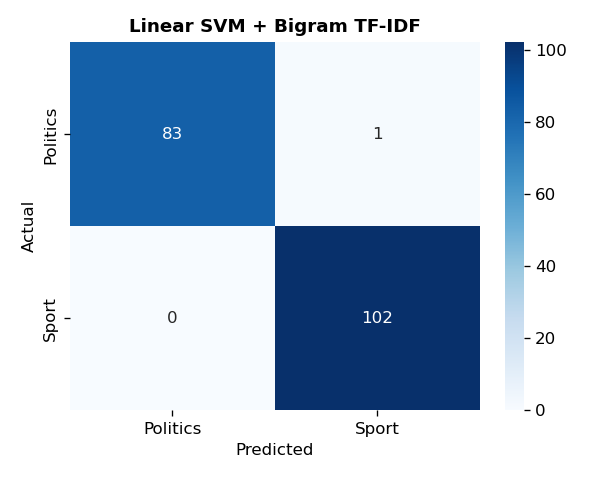
\includegraphics[width=\textwidth]{cm_Linear_SVM__Bigram_TFIDF.png}
  \caption{SVM + Bigram TF-IDF}
\end{subfigure}
\caption{Confusion matrices for LR and SVM with Bigram TF-IDF.}
\label{fig:cm_bigram}
\end{figure}

\begin{figure}[h]
\centering
\begin{subfigure}[b]{0.48\columnwidth}
  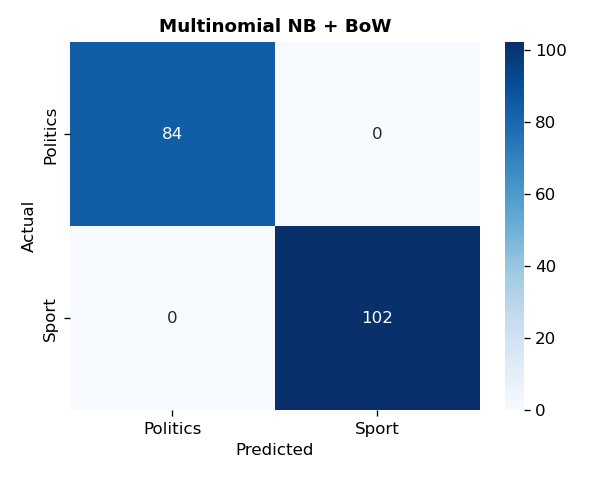
\includegraphics[width=\textwidth]{cm_Multinomial_NB__BoW.png}
  \caption{MNB + BoW}
\end{subfigure}
\hfill
\begin{subfigure}[b]{0.48\columnwidth}
  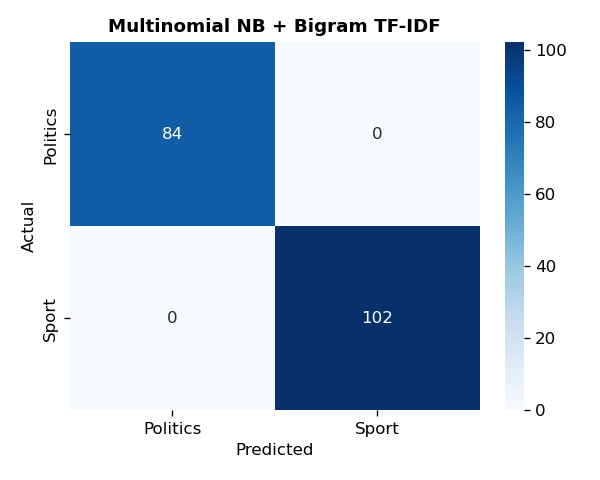
\includegraphics[width=\textwidth]{cm_Multinomial_NB__Bigram_TFIDF.png}
  \caption{MNB + Bigram TF-IDF}
\end{subfigure}
\caption{Confusion matrices for Multinomial NB with BoW and Bigram TF-IDF (both perfect).}
\label{fig:cm_mnb}
\end{figure}


% ═════════════════════════════════════════════════════════════════════════
\section{Limitations}
\label{sec:limitations}
% ═════════════════════════════════════════════════════════════════════════

\begin{enumerate}
  \item \textbf{Binary classification only.}  
  The system handles exactly two categories.  Extending to the full five BBC categories (or arbitrary taxonomies) requires further evaluation of multi-class strategies.

  \item \textbf{Domain-specific dataset.}  
  The BBC News dataset consists of formal British English news.  Performance may degrade on informal text (social media, blogs), non-English text, or news from other outlets with different editorial styles.

  \item \textbf{Small dataset.}  
  With only 928 filtered documents, the dataset is small by modern standards.  Deep learning approaches would likely need more data to be competitive.

  \item \textbf{No deep learning baseline.}  
  We compare only classical ML models.  Transformer-based models (BERT, RoBERTa) may match or exceed these results, especially on harder tasks.

  \item \textbf{Static features.}  
  BoW and TF-IDF discard word order, syntax, and deeper semantics.  Word embeddings (Word2Vec, GloVe) or contextual embeddings (BERT) capture richer representations.

  \item \textbf{No hyperparameter tuning.}  
  Default hyperparameters were used.  Grid search or Bayesian optimisation could improve results, though near-perfect accuracy limits the headroom.

  \item \textbf{Temporal bias.}  
  The dataset was collected circa 2004--2005.  Political and sporting vocabulary has evolved since then; a model trained on this data may struggle with contemporary articles.

  \item \textbf{Mild class imbalance.}  
  The 55/45 split is not severe, but severely skewed production settings would require techniques like SMOTE or class-weight adjustment.
\end{enumerate}


% ═════════════════════════════════════════════════════════════════════════
\section{Conclusion}
\label{sec:conclusion}
% ═════════════════════════════════════════════════════════════════════════

We built a complete text classification pipeline for categorising BBC news articles as Sport or Politics.
Using three feature representations (BoW, TF-IDF, Bigram TF-IDF) and three ML classifiers (Logistic Regression, Multinomial Na\"ive Bayes, Linear SVM), we conducted 9 systematic experiments.

\textbf{Multinomial Na\"ive Bayes} emerged as the best overall model, achieving \textbf{100\,\% test accuracy} with all three feature sets.
All models exceeded 98.9\,\% accuracy, demonstrating that this binary task benefits from a strong lexical separation between the two domains.

For more challenging tasks --- multi-class classification, diverse corpora, or informal text --- we recommend exploring contextual embeddings and fine-tuned transformer architectures as future directions.


% ═════════════════════════════════════════════════════════════════════════
\section{Code Availability}
% ═════════════════════════════════════════════════════════════════════════

The complete source code, dataset pipeline, and reproducible experiments are publicly available on GitHub:

\begin{center}
\url{https://github.com/kingkenche/Natural_Language_Understanding}
\end{center}

% ═════════════════════════════════════════════════════════════════════════
% REFERENCES
% ═════════════════════════════════════════════════════════════════════════

\begin{thebibliography}{5}

\bibitem{greene2006}
D.~Greene and P.~Cunningham,
``Practical Solutions to the Problem of Diagonal Dominance in Kernel Document Clustering,''
in \emph{Proc.\ 23rd International Conference on Machine Learning (ICML)}, 2006.

\bibitem{pedregosa2011}
F.~Pedregosa \emph{et al.},
``Scikit-learn: Machine Learning in Python,''
\emph{Journal of Machine Learning Research}, vol.~12, pp.~2825--2830, 2011.

\bibitem{bird2009}
S.~Bird, E.~Klein, and E.~Loper,
\emph{Natural Language Processing with Python}.
O'Reilly Media, 2009.

\bibitem{manning2008}
C.~D.~Manning, P.~Raghavan, and H.~Sch\"utze,
\emph{Introduction to Information Retrieval}.
Cambridge University Press, 2008.

\bibitem{mccallum1998}
A.~McCallum and K.~Nigam,
``A Comparison of Event Models for Naive Bayes Text Classification,''
in \emph{AAAI Workshop on Learning for Text Categorization}, 1998.

\end{thebibliography}

\end{document}
